\chapter{Loop Transformations}
\label{ch:ch19-loop-transformations}

\section{Reshaping the Hot Path}
\label{sec:ch19-reshaping}

Loop analysis tells us where loops are and how they iterate.
\term{Loop transformations} change the shape of those loops to make them cheaper.
The motivation is that loop overhead and loop structure, not just the body, cost real time.
Every iteration pays for a branch, a counter update, and often a fresh round of address arithmetic.
Memory access patterns set by the loop order decide whether each cache line serves many iterations or one.
Branches and straight-line length decide how much work the processor can overlap.
No single shape is best for every loop, so compilers reshape loops to fit the body, the bounds, and the machine.
The menu includes \term{unrolling}, which replicates the body; \term{peeling}, which separates boundary iterations; \term{fusion} and \term{fission}, which join or split loops; \term{interchange}, which swaps nesting order; and \term{tiling}, which blocks iteration space for caches.
Every transformation must preserve the order of observable effects and the values the program computes.
\term{Dependence analysis} decides legality by checking that no transformation reorders two accesses to the same location in a way the program could observe.
This chapter works through unrolling completely, surveys the remaining transformations with their legality checks, and measures each one by counting what actually changes.
It consumes the loops found in Chapter~\ref{ch:ch18-loop-analysis} and the motion machinery of Chapter~\ref{ch:ch17-code-motion}.

\section{Unrolling in Full}
\label{sec:ch19-unrolling}

\term{Loop unrolling} replicates the body $k$ times and steps the counter by $k$ per iteration, where $k$ is the \term{unroll factor}.
Listing~\ref{lst:ch19-rolled} sums one hundred elements, and Listing~\ref{lst:ch19-unrolled} shows the same loop unrolled by four.

\begin{irlisting}[caption={A simple accumulation loop with trip count one hundred.},label={lst:ch19-rolled}]
i = 0
s = 0
head: if i >= 100 goto done
      s = s + a[i]
      i = i + 1
      goto head
done: ret s
\end{irlisting}

\begin{irlisting}[caption={The same loop unrolled by four with no remainder.},label={lst:ch19-unrolled}]
i = 0
s = 0
head: if i >= 100 goto done
      s = s + a[i]
      s = s + a[i+1]
      s = s + a[i+2]
      s = s + a[i+3]
      i = i + 4
      goto head
done: ret s
\end{irlisting}

Unrolling attacks three costs at once.
Branch and counter overhead drops by a factor of $k$, because one test governs $k$ copies.
Longer straight-line bodies expose more instruction-level parallelism to the scheduler.
Redundancy across copies becomes visible to value numbering, so shared address terms merge.
The price is code size, register pressure, and a \term{remainder} problem when the trip count is not divisible by $k$.
A count of $102$ with $k = 4$ unrolls twenty-five full groups of four and leaves two extra iterations.
The compiler handles the remainder with a small cleanup loop, with peeled copies, or with a masked final iteration, depending on the target.
Algorithm~\ref{alg:ch19-unroll} states the transformation for counted loops with a cleanup loop.

\begin{algorithm}
  \caption{Unrolling a counted loop with a cleanup loop}\label{alg:ch19-unroll}
  \begin{pseudocode}
    \Require counted loop $L$, nonnegative exact trip count $T$, step $1$, integer factor $k\ge1$, safe counter arithmetic
    \Ensure body replicated $k$ times plus a loop for the remainder
    \State $full \gets \lfloor T / k \rfloor$
    \State $rem \gets T \bmod k$
    \State rewrite $L$ to iterate $full$ times with step $k$ and $k$ body copies
    \State adjust each copy $j$ to use index $i + j$ for $0 \le j < k$
    \State emit a cleanup loop of $rem$ single copies after $L$
    \State run verification that $full \cdot k + rem = T$
  \end{pseudocode}
\end{algorithm}

The algorithm assumes the trip count is known and the body contains no early exits, because an exit inside one copy would need new control flow.
The copies execute in original iteration order, preserving loop-carried dependences such as successive updates to \code{s}.
Unrolling alone does not require independence; reordering or executing the copies in parallel requires a separate dependence proof.
Dependence analysis generalizes these checks to loops with memory accesses, and the table in Section~\ref{sec:ch19-menu} lists the check each transformation needs.

\section{Worked Example: Counting What Unrolling Saves}
\label{sec:ch19-worked-counts}

We measure Listings~\ref{lst:ch19-rolled} and~\ref{lst:ch19-unrolled} by counting dynamic operations for $T = 100$ and $k = 4$.
Counting the final failed header test, the rolled loop executes $101$ tests, $100$ counter updates, $100$ loads, and $100$ additions into \code{s}.
The unrolled main loop executes $26$ tests, $25$ counter updates, $100$ loads, and $100$ additions.
With the statically empty cleanup removed, test and counter work drops from $201$ operations to $51$.
Code size grows from one body copy to four, plus the cleanup loop, which is empty here because $100 \bmod 4 = 0$.
For $T = 102$, the main loop runs $25$ iterations covering indices $0$ through $99$, and the cleanup loop runs $2$ iterations for indices $100$ and $101$.
The identity $25 \cdot 4 + 2 = 102$ confirms full coverage with no overlap.
Figure~\ref{fig:visual-unroll-tail} uses ten iterations so that every covered index fits in one diagram.
The two full groups cover $0$ through $7$; the scalar tail covers $8$ and $9$.
The boundary is a partition of the original iteration sequence, not permission to access two more array elements to fill a vector or unrolled group.

\begin{figure}[htbp]
  \centering
  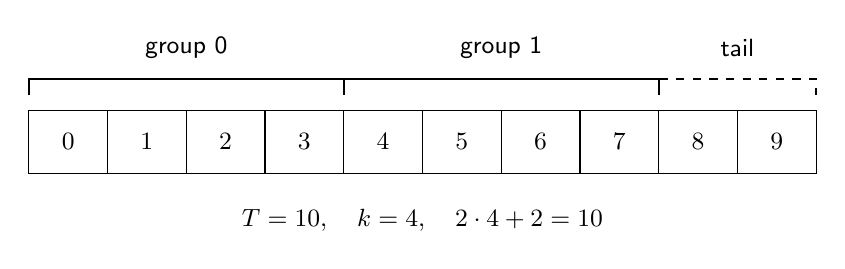
\begin{tikzpicture}[x=10mm,y=10mm]
    \foreach \i in {0,...,9} {
      \draw (\i,0) rectangle +(1,0.8);
      \node[font=\small] at (\i+0.5,0.4) {\i};
    }
    \draw[thick] (0,1) -- (0,1.2) -- (4,1.2) -- (4,1);
    \draw[thick] (4,1) -- (4,1.2) -- (8,1.2) -- (8,1);
    \draw[dashed,thick] (8,1) -- (8,1.2) -- (10,1.2) -- (10,1);
    \node[font=\sffamily\small] at (2,1.6) {group 0};
    \node[font=\sffamily\small] at (6,1.6) {group 1};
    \node[font=\sffamily\small] at (9,1.6) {tail};
    \node[font=\small] at (5,-0.6) {$T=10,\quad k=4,\quad 2\cdot4+2=10$};
  \end{tikzpicture}
  \caption{Two full groups and a two-iteration tail cover ten iterations once each, preserving their original order.}
  \label{fig:visual-unroll-tail}
\end{figure}


Engineers sometimes call the cleanup loop the \enquote{remainder loop}, and the name reminds us that its trip count is $T \bmod k$.
Table~\ref{tab:ch19-counts} records both cases.

\begin{table}
  \centering
  \caption{Dynamic operation counts for the accumulation loop rolled and unrolled by four.}
  \label{tab:ch19-counts}
  \begin{tabular}{llll}
    \toprule
    Case & Tests plus updates & Loads plus adds & Body copies \\
    \midrule
    Rolled, $T = 100$ & 201 & 200 & 1 \\
    Unrolled $k = 4$, $T = 100$ & 51 & 200 & 4 \\
    Unrolled $k = 4$, $T = 102$ & 56 including cleanup & 204 & 4 plus cleanup \\
    \bottomrule
  \end{tabular}
\end{table}

The arithmetic shows exactly what unrolling buys and what it does not.
It never reduces the essential work of loads and additions.
It reduces per-iteration overhead and lengthens the body for later passes.
Figure~\ref{fig:ch19-unrolled-shape} shows the control-flow effect: the loop keeps one header and one latch, but the body block holds four copies and the step changes.
When the scheduler later overlaps the four independent loads, the longer body turns into faster execution.
When the body already strains the registers, the same growth causes spills, and a smaller factor wins.
That tradeoff is why compilers autotune the factor or cap it by a size budget rather than unrolling maximally.

\begin{figure}
  \centering
  \begin{tikzpicture}[node distance=12mm and 22mm]
    \node[basic block] (ch19h1) {H: test i < 100};
    \node[basic block,below=of ch19h1] (ch19b1) {B: 1 copy; i = i+1};
    \node[basic block,below=of ch19b1] (ch19x1) {X: ret s};
    \draw[cfg edge] (ch19h1) -- (ch19b1);
    \draw[cfg edge] (ch19h1.east) -- ++(8mm,0) |- (ch19x1.east);
    \draw[back edge] (ch19b1.west) -- ++(-8mm,0) |- (ch19h1.west);
    \node[basic block,right=30mm of ch19h1] (ch19h2) {H: test i < 100};
    \node[basic block,below=of ch19h2] (ch19b2) {B: 4 copies; i = i+4};
    \node[basic block,below=of ch19b2] (ch19x2) {X: ret s};
    \draw[cfg edge] (ch19h2) -- (ch19b2);
    \draw[cfg edge] (ch19h2.east) -- ++(8mm,0) |- (ch19x2.east);
    \draw[back edge] (ch19b2.west) -- ++(-8mm,0) |- (ch19h2.west);
    \node[font=\sffamily\small,above=4mm of ch19h1] {Before};
    \node[font=\sffamily\small,above=4mm of ch19h2] {After};
  \end{tikzpicture}
  \caption{Unrolling by four keeps the loop skeleton and quadruples the body, so one test governs four loads and four additions.}
  \label{fig:ch19-unrolled-shape}
\end{figure}

\section{A Menu of Transformations}
\label{sec:ch19-menu}

Unrolling is one entry in a larger menu, and Table~\ref{tab:ch19-menu} surveys the rest with the payoff and legality check for each.
\term{Loop peeling} separates the first or last few iterations from the steady state.
It aligns the loop for vectorization, removes a boundary test from the hot path, or pairs a warm-up iteration with following code.
Its legality check is that the peeled copies execute under the same conditions as the original iterations.
\term{Loop fusion} merges two adjacent loops over the same range into one loop with both bodies.
It halves loop overhead and keeps shared data in registers or caches between the two bodies.
It is legal when no dependence flows backward across the merge, meaning the second loop must not read values the first loop writes in a later iteration than the read.
\term{Loop fission}, also called distribution, splits one loop into several for the mirror reason: separating heavy bodies can improve locality, enable vectorization of one part, or isolate a serial section.
Its check is the reverse, namely that no dependence needed within one iteration is broken by the split.
\term{Loop interchange} swaps an inner loop with an outer one.
It converts strided access into sequential access, which is often the largest cache win available, and it can move a parallelizable loop outward.
It is legal when the dependence direction permits the swap, which the compiler tests with direction vectors over the iteration space.
\term{Loop tiling}, also called blocking, partitions iterations into blocks sized for a cache level.
It reuses each loaded line many times before eviction and is the standard treatment for matrix codes.
Its legality generalizes interchange to strip-mined bands, and its block sizes come from machine parameters rather than from the source.
% TODO(cite): primary references for dependence testing and tiling legality.

\begin{table}
  \centering
  \caption{Common loop transformations with their main payoff and the legality check each one requires.}
  \label{tab:ch19-menu}
  \begin{tabular}{lll}
    \toprule
    Transformation & Main payoff & Legality check \\
    \midrule
    Unrolling & Less overhead, longer bodies & Known count, no early exits \\
    Peeling & Aligned steady state & Same conditions for split copies \\
    Fusion & Shared data stays hot & No backward dependence across merge \\
    Fission & Separated concerns vectorize & No split of a needed ordering \\
    Interchange & Sequential memory access & Dependence direction permits swap \\
    Tiling & Cache-level reuse & Bands respect all dependences \\
    \bottomrule
  \end{tabular}
\end{table}

Transformations compose, and order matters.
Peeling before vectorization, interchange before tiling, and unrolling after everything else is a common pipeline.
Each step must update the loop tree and any cached dependence facts, or the next step reasons from stale structure.

\section{Implementation Notes}
\label{sec:ch19-implementation}

Unrolling a body of size $B$ by factor $k$ costs $O(k \cdot B)$ time and produces $O(k \cdot B)$ code, plus the cleanup loop.
There are $O(d^2)$ candidate pairs for $d$ memory references; the cost of solving each dependence query must be counted in addition to enumerating pairs.
Tiling and interchange add polyhedral-style reasoning whose worst case is exponential in loop depth, so production compilers apply exact tests only to small depths and profitable-looking loops.
% TODO(cite): primary reference for the dependence-test complexity bounds.
Profitability heuristics dominate practice.
Compilers unroll small counted loops fully, partially unroll hot loops by factors from four to sixteen, and refuse when the body already exceeds a size or pressure budget.
They tile only loops whose working sets exceed a cache level but fit when blocked, using machine parameters for line size and capacity.
They fuse when the merged body fits comfortably and fission when separation unlocks vectorization.
Every transformation preserves a verification hook: trip-count identities like $full \cdot k + rem = T$, bounds recomputed from the original, and dependence rechecks after rewriting.
Keep those hooks even in a teaching compiler, because loop bugs corrupt many iterations from one wrong decision.

\begin{ccnote}[Order effects]
Unrolling before redundancy removal finds cross-copy common expressions, while motion before unrolling shrinks the body that gets replicated.
Run invariant motion first, then unroll, then run numbering and scheduling again on the longer body.
\end{ccnote}

\section{Exercises}
\label{sec:ch19-exercises}

\begin{enumerate}
  \item \label{ex:ch19-remainder}
  Unroll Listing~\ref{lst:ch19-rolled} by $k = 4$ for $T = 103$ using Algorithm~\ref{alg:ch19-unroll}.
  Give $full$ and $rem$, write the resulting IR including the cleanup loop, and verify the coverage identity.
  Count dynamic tests, updates, loads, and additions, and state how many iterations the cleanup loop runs.
  \item \label{ex:ch19-fusion-check}
  Give two adjacent loops over the same index range where the first writes \code{a[i]} and the second reads \code{a[i-1]}.
  Decide whether fusion is legal by tracing the dependence from the write in iteration $i$ to the read in iteration $i+1$.
  Show the fused body, state which iteration pair creates the backward dependence, and give the verdict with the reason.
  \item \label{ex:ch19-interchange-win}
  Give a doubly nested loop that reads \code{m[i][j]} with row-major storage where the inner loop varies \code{i}.
  Compute the stride of consecutive inner iterations in units of elements, then interchange the loops and recompute the stride.
  Explain which version reuses each cache line fully and what dependence fact would forbid the swap.
\end{enumerate}

\section{Further reading}
\label{sec:ch19-further-reading}

Morgan's \emph{Building an Optimizing Compiler} covers loop restructuring among the optimizations that change control flow~\cite{morgan-1998-optimizing}.
Read it for how legality checks gate each transformation.
Appel's \emph{Modern Compiler Implementation in ML} shows the loop analyses that transformations depend on~\cite{appel-1998-modern}.
Use it to connect the loop tree of Chapter~\ref{ch:ch18-loop-analysis} to the rewrites here.
The C11 committee draft defines the observable behavior that limits reordering of memory accesses~\cite{wg14-2011-c11}.
Consult its rules on sequencing and volatile access before moving any load or store across a loop boundary.
